\section[Problema 3]{Problema 3}

Nesse problema do caxeiro viajante, o algoritmo Hill-Climbing com restart se destacou, apresentando os melhores resultados entre todos os demais algoritmos, o Simulated Annealing também apresentou uma performance muito parecida, logo seguido do algoritmo do Hill-Climbing, no entanto o GA chegou apenas a alcançar o mínimo local de 15008, ainda que seja um valor muito longe do mínimo global, que é de 6656, observamos que esse algoritmo ainda não havia chegado ao seu potencial máximo, pois os valores de novas populações ainda estavam oscilando muito, como pode ser visto na figura \ref{fig:problema-3-genetic-algorithm-funcao-objetivo-value}, se compararmos com as figuras dos problemas anteriores \ref{fig:problema-1-genetic-algorithm-funcao-objetivo-value} e \ref{fig:problema-2-genetic-algorithm-funcao-objetivo-value}, vemos claramente que mesmo após 100k iterações os valores atuais ainda não haviam convergido para um valor único, enquanto nos demais problemas essa convergência ocorreu pouco após a iteração 200. \\

O algoritmo Hill-Climbing com restart além de possuir um peso computacional bem baixo, também apresentou uma eficácia grande em driblar os mínimos locais. O algoritmo genético além de possuir um peso computacional muito elevado, também apresentou uma baixa eficiência em sair dos mínimos locais, acreditamos que após algumas análises sobre esse problema que a aplicação de algumas heurísticas para melhorar a eficácia não só desse mas de todos os demais seja um caminho mais adequado, por exemplo evitando que path's cruzem com outros, verificamos que em geral a rota que segue o perímetro mais externo dos pontos, possui a distância mais curta. \\

O algoritmo Hill-Climbing apresentou boa performance para esse problema e conseguiu ao longo das iterações fugir de mínimos locais, apesar de ficar um pouco distante dos algoritmos Hill-Climbing com restart e Simulated Annealing que apresentaram um comportamento muito parecido com números muito similares. \\

\subsection{Algoritmo Hill-Climbing}

\begin{figure}[H]
\centering
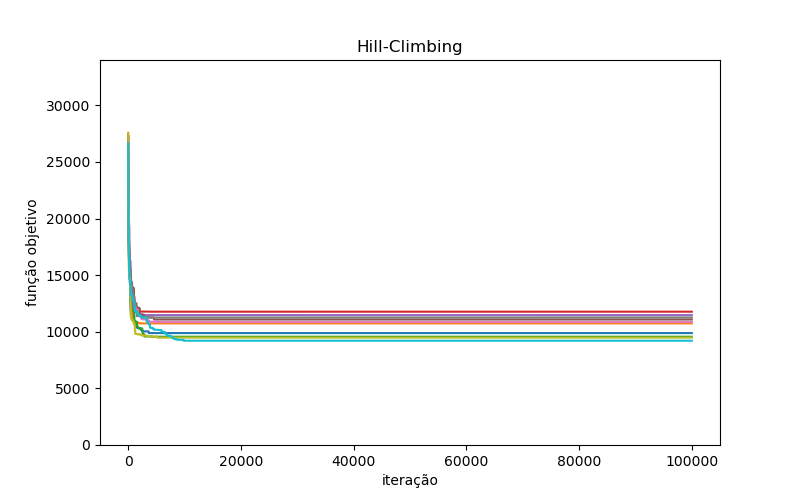
\includegraphics[width=110mm]{imagens/otima/problema-3-hill-climbing-funcao-objetivo-best.png}
\caption{Dados da execução da função objetivo durante as 10 iterações.
\label{fig:problema-3-hill-climbing-funcao-objetivo}}
\end{figure}

\subsection{Algoritmo Hill-Climbing com Restart}

\begin{figure}[H]
\centering
  \begin{minipage}[b]{0.48\textwidth}
    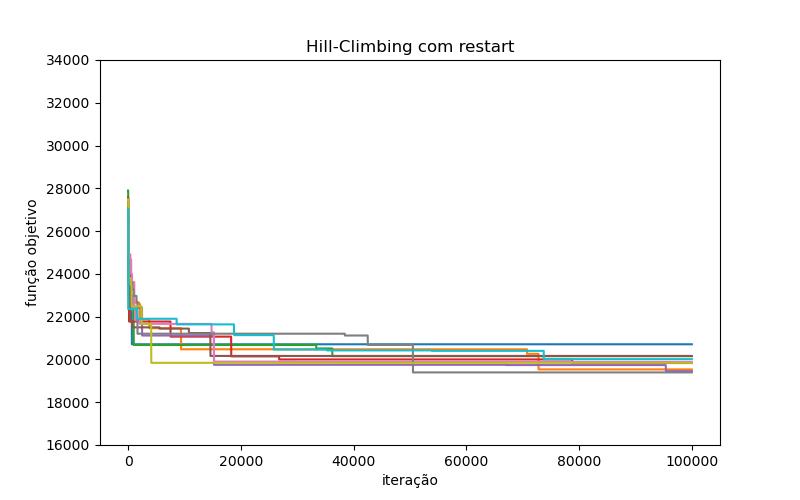
\includegraphics[width=88mm]{imagens/otima/problema-3-hill-climbing-com-restart-funcao-objetivo-best.png}
    \caption{Dados da execução da função objetivo durante as 10 iterações por melhor valor.
    \label{fig:problema-3-hill-climbing-com-restart-funcao-objetivo-best}}
  \end{minipage}
  \hfill
  \begin{minipage}[b]{0.48\textwidth}
    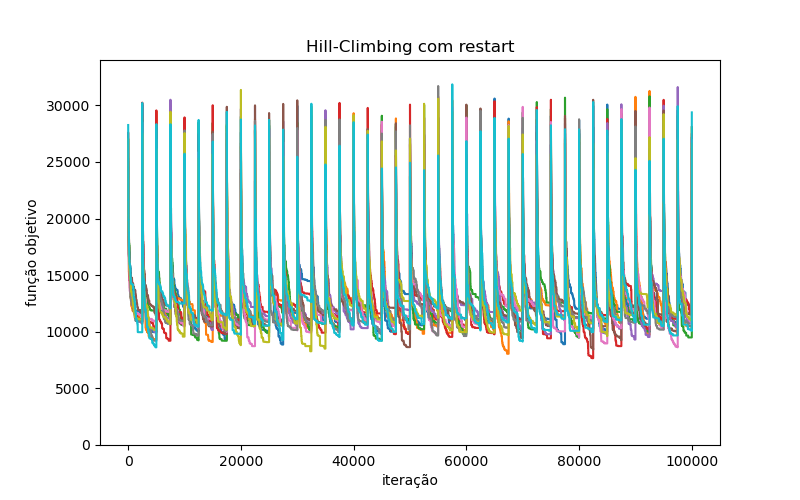
\includegraphics[width=88mm]{imagens/otima/problema-3-hill-climbing-com-restart-funcao-objetivo-value.png}
    \caption{Dados da execução da função objetivo durante as 10 iterações por valor atual.
    \label{fig:problema-3-hill-climbing-com-restart-funcao-objetivo-value}}
  \end{minipage}
\end{figure}

\subsection{Simulated Annealing}

\begin{figure}[H]
\centering
  \begin{minipage}[b]{0.48\textwidth}
    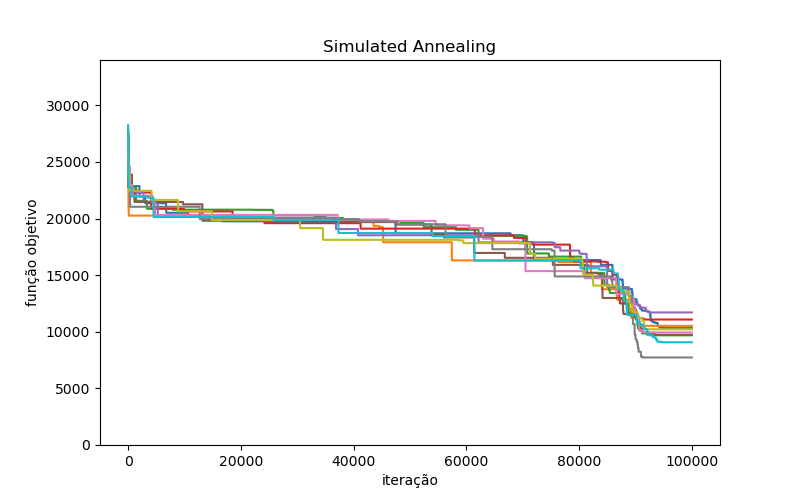
\includegraphics[width=88mm]{imagens/otima/problema-3-simulated-annealing-funcao-objetivo-best.png}
    \caption{Dados da execução da função objetivo durante as 10 iterações por melhor valor.
    \label{fig:problema-3-simulated-annealing-funcao-objetivo-best}}
  \end{minipage}
  \hfill
  \begin{minipage}[b]{0.48\textwidth}
    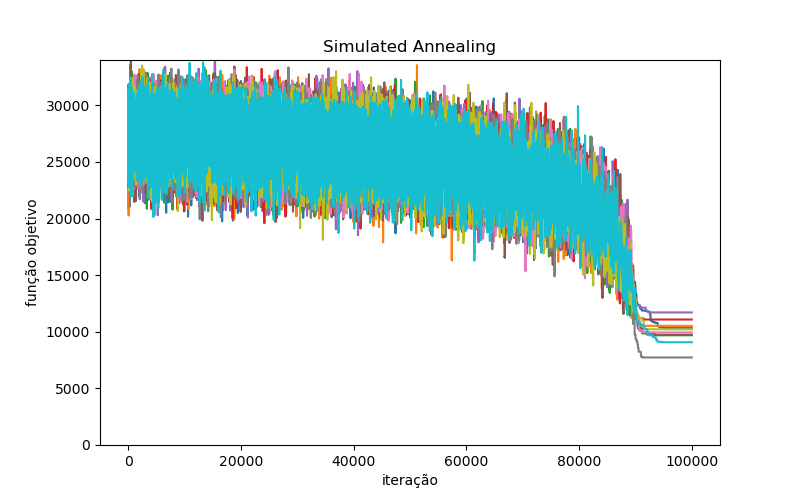
\includegraphics[width=88mm]{imagens/otima/problema-3-simulated-annealing-funcao-objetivo-value.png}
    \caption{Dados da execução da função objetivo durante as 10 iterações por valor atual.
    \label{fig:problema-3-simulated-annealing-funcao-objetivo-value}}
  \end{minipage}
\end{figure}

\subsection{Algoritmo Genético}

\begin{figure}[H]
\centering
  \begin{minipage}[b]{0.48\textwidth}
    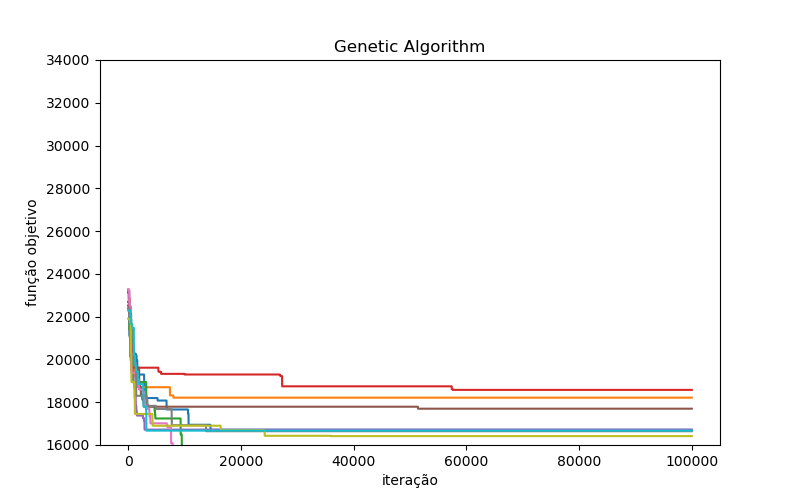
\includegraphics[width=88mm]{imagens/otima/problema-3-genetic-algorithm-funcao-objetivo-best.png}
    \caption{Dados da execução da função objetivo durante as 10 iterações por melhor valor.
    \label{fig:problema-3-genetic-algorithm-funcao-objetivo-best}}
  \end{minipage}
  \hfill
  \begin{minipage}[b]{0.48\textwidth}
    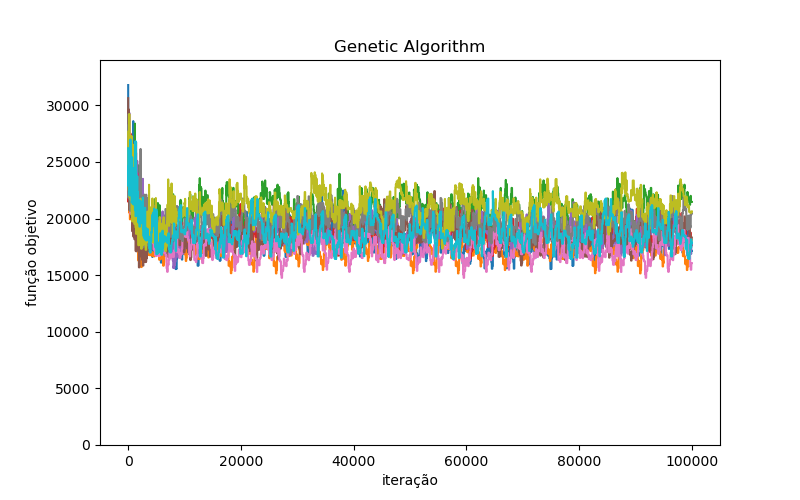
\includegraphics[width=88mm]{imagens/otima/problema-3-genetic-algorithm-funcao-objetivo-value.png}
    \caption{Dados da execução da função objetivo durante as 10 iterações por valor atual.
    \label{fig:problema-3-genetic-algorithm-funcao-objetivo-value}}
  \end{minipage}
\end{figure}